\documentclass[10pt]{article}
\usepackage[utf8]{inputenc}
\usepackage[T1]{fontenc}
\usepackage[margin=0.95in]{geometry}
\usepackage{amsmath,amssymb,amsthm}
\usepackage{booktabs}
\usepackage{array}
\usepackage{url}
\usepackage{microtype}
\usepackage{graphicx}
\usepackage{caption}
\usepackage{xcolor}
\usepackage{listings}
\usepackage[hidelinks]{hyperref}
\makeatletter\g@addto@macro{\UrlBreaks}{\do\_\do\.\do\/}\makeatother
\emergencystretch=3em
\tolerance=2000
% generated by gen_inputs.py; do not edit
\newcommand{\ZPBrFour}{+5.404\times10^{-5}}
\newcommand{\ZPBrOne}{+4.220\times10^{-5}}
\newcommand{\ZPBrThree}{-7.064\times10^{-5}}
\newcommand{\ZPBrTwo}{-4.279\times10^{-5}}
\newcommand{\ZPBugDropMax}{17.7}
\newcommand{\ZPBugDropMin}{0.027}
\newcommand{\ZPBugSwapOneMax}{1.1\times10^{-15}}
\newcommand{\ZPBugSwapOtherMax}{9.4}
\newcommand{\ZPBugSwapOtherMin}{0.904}
\newcommand{\ZPCargoFailed}{0}
\newcommand{\ZPCargoIgnored}{1}
\newcommand{\ZPCargoPassed}{59}
\newcommand{\ZPCitationAccepted}{3}
\newcommand{\ZPCitationN}{3}
\newcommand{\ZPConcOne}{-3.048}
\newcommand{\ZPCurvNA}{21}
\newcommand{\ZPCutoffMax}{2.2\times10^{-13}}
\newcommand{\ZPDecompResid}{6.5\times10^{-5}}
\newcommand{\ZPDipEwaldMax}{3.89\times10^{-7}}
\newcommand{\ZPDroppedGaussHalf}{-3.81\times10^{-4}}
\newcommand{\ZPDroppedYuk}{-9.50\times10^{-4}}
\newcommand{\ZPElasticRcDiff}{9.0\times10^{-7}}
\newcommand{\ZPElenchusSeedRc}{2}
\newcommand{\ZPEpsteinMax}{3.89\times10^{-7}}
\newcommand{\ZPEpsteinMaxHi}{9.7\times10^{-10}}
\newcommand{\ZPEzpHead}{1.4902783183}
\newcommand{\ZPEzpTri}{1.5033523522}
\newcommand{\ZPFrozenMax}{2.14\times10^{-7}}
\newcommand{\ZPFrozenN}{33}
\newcommand{\ZPGateBlock}{0}
\newcommand{\ZPGateExit}{1}
\newcommand{\ZPGateFlag}{8}
\newcommand{\ZPGateFlagKinds}{LEDGER\_UNAUDITED\_TIER\_A}
\newcommand{\ZPGaussTwoCtl}{+4.533\times10^{-3}}
\newcommand{\ZPGaussTwoUnstableA}{unstable}
\newcommand{\ZPGaussTwoUnstableB}{unstable}
\newcommand{\ZPHumanDiffDuffy}{4.3\times10^{-12}}
\newcommand{\ZPHumanHead}{1.490278318}
\newcommand{\ZPHumanRatioHead}{0.068}
\newcommand{\ZPHumanRatioTri}{0.097}
\newcommand{\ZPHumanSq}{-0.1441}
\newcommand{\ZPHumanTri}{1.503352352}
\newcommand{\ZPHumandE}{-1.3074\times10^{-2}}
\newcommand{\ZPIndepGaussTri}{1.5033524}
\newcommand{\ZPIsoGradMax}{1.5\times10^{-6}}
\newcommand{\ZPIsoGradQuarter}{1.2\times10^{-5}}
\newcommand{\ZPIsoRelMax}{1.5\times10^{-6}}
\newcommand{\ZPIsoRelQuarter}{4.3\times10^{-4}}
\newcommand{\ZPIsoXYMax}{2.0\times10^{-8}}
\newcommand{\ZPKgridErrMax}{6.5\times10^{-6}}
\newcommand{\ZPKgridErrMin}{2.6\times10^{-8}}
\newcommand{\ZPKgridErrOne}{1.3\times10^{-6}}
\newcommand{\ZPKgridExpMax}{3.01}
\newcommand{\ZPKgridExpMin}{3.00}
\newcommand{\ZPLWHead}{0.1047}
\newcommand{\ZPLWHeadExact}{0.1047}
\newcommand{\ZPLWSqGaussOne}{-0.1475}
\newcommand{\ZPLWTri}{0.2383}
\newcommand{\ZPLWTriExact}{0.2383}
\newcommand{\ZPLambdaFirstMax}{10.0}
\newcommand{\ZPLambdaFirstMin}{0.1}
\newcommand{\ZPLambdaSurviveAll}{all five}
\newcommand{\ZPLapOne}{-3.848}
\newcommand{\ZPLargestRobust}{-5.12\times10^{-2}}
\newcommand{\ZPLeanCtlAxiom}{yes}
\newcommand{\ZPLeanCtlSorryAx}{yes}
\newcommand{\ZPLeanCtlWrongOk}{yes}
\newcommand{\ZPLeanNInAllow}{19}
\newcommand{\ZPLeanNThm}{19}
\newcommand{\ZPLeanRc}{0}
\newcommand{\ZPLeanRerunCtlRc}{0}
\newcommand{\ZPLeanRerunRc}{0}
\newcommand{\ZPLeanRerunSameBasic}{identical to}
\newcommand{\ZPLeanRerunSameCtl}{identical to}
\newcommand{\ZPLeanRerunSecs}{7.9}
\newcommand{\ZPLeanSecs}{8.5}
\newcommand{\ZPLeanSorryCount}{0}
\newcommand{\ZPLedgerA}{8}
\newcommand{\ZPLedgerC}{13}
\newcommand{\ZPLedgerL}{3}
\newcommand{\ZPLedgerN}{37}
\newcommand{\ZPLedgerX}{13}
\newcommand{\ZPLinOne}{-0.799}
\newcommand{\ZPListRefuted}{\texttt{dipolar:0.1}, \texttt{dipolar:0.5}, \texttt{gauss:0.5}, \texttt{gauss:1}, \texttt{riesz:3}, \texttt{riesz:4}, \texttt{yukawa:1}, \texttt{yukawa:2}}
\newcommand{\ZPListSurvive}{\texttt{gauss:0.25}, \texttt{gauss:2}, \texttt{gauss:4}, \texttt{riesz:6}}
\newcommand{\ZPMapMaxdE}{-1.3\times10^{-4}}
\newcommand{\ZPMapNComp}{64}
\newcommand{\ZPMapNLower}{64}
\newcommand{\ZPMapNShapes}{625}
\newcommand{\ZPMapNStable}{65}
\newcommand{\ZPMargConv}{3.3\times10^{-9}}
\newcommand{\ZPMargFrac}{0.06}
\newcommand{\ZPMargLW}{1.317\times10^{-4}}
\newcommand{\ZPMarginRatio}{10052}
\newcommand{\ZPMaxStableDist}{0.23}
\newcommand{\ZPModularMax}{2.2\times10^{-13}}
\newcommand{\ZPNRefuted}{8}
\newcommand{\ZPNScanPoints}{567}
\newcommand{\ZPNStableGaussOne}{16}
\newcommand{\ZPNSurvive}{4}
\newcommand{\ZPNTested}{12}
\newcommand{\ZPNTwoComp}{7}
\newcommand{\ZPNoTwoComp}{\texttt{riesz:4}}
\newcommand{\ZPPoissonRealMax}{1.4\times10^{-14}}
\newcommand{\ZPQuadErr}{4.4\times10^{-15}}
\newcommand{\ZPRatioHead}{0.03493}
\newcommand{\ZPRatioMarg}{1.317\times10^{-4}}
\newcommand{\ZPRatioTri}{0.03222}
\newcommand{\ZPRerunC}{-0.961984}
\newcommand{\ZPRerunEzpHead}{1.490278318280}
\newcommand{\ZPRerunEzpTri}{1.503352352207}
\newcommand{\ZPRerundE}{-1.3074\times10^{-2}}
\newcommand{\ZPReviseCargoFailed}{0}
\newcommand{\ZPReviseCargoIgnored}{1}
\newcommand{\ZPReviseCargoPassed}{60}
\newcommand{\ZPRootA}{0.123}
\newcommand{\ZPRootLapm}{1.09361}
\newcommand{\ZPRootOne}{0.37668}
\newcommand{\ZPRootTwo}{1.58148}
\newcommand{\ZPRustDiffHead}{2.6\times10^{-9}}
\newcommand{\ZPRustDiffTri}{2.5\times10^{-9}}
\newcommand{\ZPRustHead}{1.490278316}
\newcommand{\ZPRustTri}{1.503352350}
\newcommand{\ZPRustyEdge}{5f2f73b8c636c4ae45a43ad67c99621acc609660}
\newcommand{\ZPRustyEdgeShort}{5f2f73b}
\newcommand{\ZPRustyGate}{a961a714dd040ad1e1a542db1efc54e0401cd55b}
\newcommand{\ZPRustyGateShort}{a961a71}
\newcommand{\ZPRustyHarden}{609338e6485fc96002e4c60c0c3e34f9130c0108}
\newcommand{\ZPRustyHardenShort}{609338e}
\newcommand{\ZPRustySpectral}{6ad3cf7e5e171479d1481e5fd17e7d432aae21d1}
\newcommand{\ZPRustySpectralShort}{6ad3cf7}
\newcommand{\ZPShaBasic}{7d59f1817767ae64cc37d017348e1eb5f5b9ed83ed068086fae839baff0d64f0}
\newcommand{\ZPShaCtl}{c725bdcba93362681c58f65eaf00d717eea37254c10f364bab4e039d645acd90}
\newcommand{\ZPShaMatch}{match}
\newcommand{\ZPShellFracOne}{63}
\newcommand{\ZPSmallaAFifteenRatio}{1.7\times10^{-7}}
\newcommand{\ZPSmallaAHundred}{-0.0062}
\newcommand{\ZPSmallaTriLam}{3.3\times10^{-12}}
\newcommand{\ZPSplitDtrD}{-2.033\times10^{-2}}
\newcommand{\ZPSplitEinstein}{-3.131\times10^{-3}}
\newcommand{\ZPSplitEinsteinPct}{24}
\newcommand{\ZPSplitJensen}{-9.943\times10^{-3}}
\newcommand{\ZPSplitJensenPct}{76}
\newcommand{\ZPSplitLower}{-1.751\times10^{-2}}
\newcommand{\ZPSplitLowerLW}{-1.33\times10^{-5}}
\newcommand{\ZPSplitLowerMid}{-2.527\times10^{-3}}
\newcommand{\ZPSplitLowerZB}{-1.497\times10^{-2}}
\newcommand{\ZPSplitTwoDtrD}{5.393\times10^{-2}}
\newcommand{\ZPSplitTwoTotal}{4.533\times10^{-3}}
\newcommand{\ZPSplitTwoUpper}{2.440\times10^{-2}}
\newcommand{\ZPSplitUpper}{4.436\times10^{-3}}
\newcommand{\ZPSqUnstable}{-0.1475}
\newcommand{\ZPStaticTriAll}{all 12}
\newcommand{\ZPSumRuleDuffyMax}{2.7\times10^{-14}}
\newcommand{\ZPSumRuleMaxErr}{3.0\times10^{-16}}
\newcommand{\ZPSumRuleMtwoErr}{5.1\times10^{-16}}
\newcommand{\ZPSumRuleNPts}{5}
\newcommand{\ZPSumRulePRMax}{5.9\times10^{-15}}
\newcommand{\ZPSumRuleThetaHex}{1.1595952670}
\newcommand{\ZPVoneRatio}{-3.24\times10^{-5}}
\newcommand{\ZPWellsSqStable}{stable}
\newcommand{\ZPWellsStatic}{-0.506}
\newcommand{\ZPWellsTwoZp}{-2.04}
\newcommand{\ZPWellsZp}{-3.03}
\newcommand{\ZPcFour}{+0.313}
\newcommand{\ZPcHalf}{-0.461}
\newcommand{\ZPcOne}{-0.962}
\newcommand{\ZPcQuarter}{+0.188}
\newcommand{\ZPcTwo}{+0.495}
\newcommand{\ZPdEHead}{-1.3074\times10^{-2}}
\newcommand{\ZPdEHeadShort}{-1.31\times10^{-2}}
\newcommand{\ZPdEMarg}{-5.123\times10^{-2}}
\newcommand{\ZPdEthree}{-4.867\times10^{-2}}

\lstset{basicstyle=\ttfamily\footnotesize,columns=fullflexible,keepspaces=true,breaklines=true,
  frame=single,framesep=3pt,xleftmargin=4pt,xrightmargin=4pt,upquote=true,aboveskip=4pt,belowskip=2pt,
  keywordstyle=\bfseries,morekeywords={theorem,lemma,def,noncomputable,abbrev,where,fun,Prop,axiom},
  escapeinside={(*@}{@*)}}
\newcommand{\R}{\mathbb{R}}
\newcommand{\tier}[1]{\textsf{[#1]}}
\newcommand{\lean}[1]{\texttt{#1}}
\newcommand{\Ezp}{E_{\mathrm{zp}}}
\newcommand{\tr}{\operatorname{tr}}
\makeatletter\newcommand{\tabinput}[1]{\@@input #1 }\makeatother

\title{Does the triangular lattice minimise the harmonic zero-point energy?\\
A numerical counterexample for completely monotone potentials,\\
with kernel-checked curvature identities}
\author{Xavier Callens (SocrateAI Lab)}
\date{Preprint v1, 2026-10-25}
\hypersetup{pdftitle={Does the triangular lattice minimise the harmonic zero-point energy? A numerical counterexample},
  pdfauthor={Xavier Callens}}

\begin{document}
\maketitle
\begin{center}\small Zenodo DOI to be assigned on release \quad (not peer reviewed)\end{center}

\noindent\textbf{AI-assistance disclosure.} This preprint, its Lean code, its Rust and Python code and its claim ledger were
produced by AI agents (Claude, Anthropic) under the author's direction. The author is responsible for the content. No human
has audited the Lean statements for adequacy, and no human referee has checked the hand arguments. The paper-stage rerun of the Lean
module and of the crate tests was made by the same pipeline (Section~\ref{sec:lean}), which is not a producer~$\neq$~verifier check.
A \emph{separate} AI agent (Claude, an audit stage with its own code; \texttt{AUDIT.md}, verdict ``accept with corrections''; its corrections are applied here, see \texttt{REVISION.md})
audited the preprint within the scope stated in Section~\ref{sec:audit}. That is an AI audit, not a human audit.

\begin{abstract}
For a pair potential $V(r)=g(r^2)$ and a planar Bravais lattice of covolume one, the harmonic zero-point energy is
$\Ezp=\tfrac12\langle\sum_j\omega_j(\mathbf k)\rangle_{\mathrm{BZ}}$. Planar universal optimality (the Cohn--Kumar conjecture, a theorem for Gaussians by Montgomery; its general proof in openai/math is AI-generated and not peer reviewed) says that the
triangular lattice minimises the \emph{static} energy for every completely monotone $g$. The natural quantum analogue,
conjecture \textbf{QU-1}, says it also minimises $\Ezp$ among unit-covolume planar Bravais lattices. We tested it before
trying to prove it, and it fails numerically (Tier~X, below): we do not claim a proof that it is false.

\textbf{Tier X (floating point).} For the Gaussian $g(t)=e^{-\pi t}$, the rhombic lattice $\tau=0.5+0.966025\,i$ is
dynamically stable and has $\Delta\Ezp=\ZPdEHeadShort$ relative to the triangular lattice ($\Ezp=\ZPEzpHead$ against
$\ZPEzpTri$). Two formulas in four implementations agree: a real-space folded-grid Rust code and an independent numpy
re-implementation of it; a reciprocal-space (Poisson) Rust code with a spectrally convergent zone rule (quadrature error about
$\ZPQuadErr$); and a short third Poisson implementation in numpy. The conjecture is numerically refuted for $\ZPNRefuted$ of $\ZPNTested$ completely monotone
potentials tested (Gaussian, Yukawa, dipolar-exciton, Riesz). One of the eight, \texttt{riesz:4}, is weak: it rests on a single competitor whose exact long-wave margin is
0.08\,\% of the triangular value, its finite-$\mathbf k$ stability comes from the G1 grids only, and its triangular point is a local minimum ($c>0$).
Four potentials (Gaussian $a=0.25,2,4$ and Riesz $s=6$) are not refuted, on a sample
and two dense paths, which is not an exhaustive search. At the triangular point the curvature of $\Ezp$ is isotropic and, for the
Gaussian $e^{-\pi a r^2}$, numerically negative on $a\in(\ZPRootOne,\ZPRootTwo)$ among $0.15\le a\le4$ (a scan of 23 values of $a\in[0.1,8]$ followed by bisection of the sign changes; gaps between scan points are not excluded).

\textbf{Tier A (Lean~4.34.1, Mathlib; axioms within $\{$\lean{propext}, \lean{Classical.choice}, \lean{Quot.sound}$\}$;
planted \lean{sorry} and planted-axiom controls caught).} \ZPLeanNThm{} finite and algebraic statements: derivatives and
Laplacian identities of the lattice-vector length $Q$, the Gaussian curvature densities, the 120-degree rotation lemmas
that force an isotropic Hessian at $\rho=e^{i\pi/3}$, and an inversion step for the mean-square frequency sum rule. They
certify none of the statements about $\Ezp$.

\textbf{Tiers L and C.} Cited: Montgomery's theorem (via Deng--Luo) and two results of Luo--Wei, with the Elenchus
citation gate accepting the three quotations. Human arguments: the sum rule $\langle\tr D\rangle=4\pi a-(4\pi^2/a)S(1/a)$, the
Einstein bound, and a concavity decomposition of the curvature. No result here rests on openai/math, apart from the pinned
toolchain. We claim no proof of anything about $\Ezp$ and no breakthrough; the contribution is a negative result with
controls, and a restricted conjecture QU-1$'$ (Tier X-supported) for a range of Gaussians.
\end{abstract}

\paragraph{Tiers.} \tier{A}: kernel-checked Lean, axioms within the allowlist, planted controls caught. \tier{L}: a cited source,
quoted in the ledger and run through the Elenchus citation gate. \tier{C}: an argument or human proof that is not
machine-checked. \tier{X}: floating-point exploration, which never supports a claim by itself. Identifiers such as
\texttt{ZP-X-0001} refer to \texttt{ledger/ledger.json} (Section~\ref{sec:ledger}). A Tier~A tag attaches to the Lean statement,
never to its physical gloss. Statements about $\Ezp$ are Tier~X or~C throughout.

%=====================================================================
\section{Setting, the conjecture, and what was preregistered}\label{sec:setting}
\paragraph{The functional.} Let $L_\tau$ be the planar lattice of shape $\tau=x+iy$ ($y>0$) with basis
$a_1=(1/\sqrt y,0)$, $a_2=(x/\sqrt y,\sqrt y)$, covolume one. Particles of unit mass sit on $L_\tau$ and interact by
$V(r)=g(r^2)$ (units $\hbar=m=1$). In the harmonic approximation
\[D(\mathbf k)=\sum_{R\in L\setminus 0}(1-\cos\mathbf k\!\cdot\! R)\,\mathrm{Hess}\,V(R),\qquad
\omega_j(\mathbf k)=\sqrt{\lambda_j(D(\mathbf k))},\qquad
\Ezp(\tau)=\tfrac12\Bigl\langle\sum_{j=1}^{2}\omega_j\Bigr\rangle_{\mathrm{BZ}}\ \ \tier{C, ZP-C-0001}.\]
A lattice is \emph{dynamically stable} if $D(\mathbf k)\succeq0$ for all $\mathbf k$. $\Ezp$ is invariant under
$\tau\mapsto\tau+1$ and $\tau\mapsto-1/\tau$ (the lattice is unchanged up to rotation), which we tested numerically.

\paragraph{Conjecture QU-1 (zero-point version of triangular optimality).} For every completely monotone $g$ (a positive
mixture of $e^{-ut}$ in $t=r^2$), the triangular lattice $\rho=e^{i\pi/3}$ minimises $\Ezp(\tau)$ over unit-covolume planar
Bravais lattices. It was proposed in the programme document of 2026-10-25 as a quantum companion of planar universal
optimality (the static statement, Cohn--Kumar; its proof by the openai/math release is AI-generated and not peer reviewed,
and nothing here depends on it). The static statement for the Gaussian is Montgomery's theorem~\cite{mont,dengluo}
\tier{L, ZP-L-0003}. QU-1 was preregistered with a prior of $0.6$ that it survives a falsification gate (G1), to be followed by a
proof attempt for Gaussians (G2) \emph{only if} G1 survived.

\paragraph{What happened, and deviations from the preregistration.} G1 numerically refuted QU-1 (Tier~X). G2 as preregistered was therefore not run.
What was run under the label G2 (an independent re-verification of the counterexample, the curvature scan, the mechanism
analysis and the Lean module) is \textbf{post hoc}: the re-verification is a robustness check, while the scan of $c(a)$, its
sign changes, the decomposition and QU-1$'$ are exploratory and were not preregistered. Further deviations: (i) \emph{unstable-lattice
policy.} A lattice with any eigenvalue of $D$ below $-10^{-9}$ times the scale is dynamically unstable and its $\Ezp$ is set
to NaN and excluded; no clipping of imaginary frequencies is used for any verdict (a competitor-favouring clipped value is
reported only in the data files). The policy is a scope decision made at G1. (ii) The preregistration asked for a neutralising background
for long-range potentials; Coulomb (Riesz $s=1$) and Keldysh need a plasmon treatment of $k\to0$ that the code does not have, so
they are \emph{excluded} and nothing is claimed for them. The dipolar-exciton and Riesz $s>2$ potentials are untruncated with
$1/r^3$ or faster tails, for which no background is needed. (iii) The Lean module and this paper were not preregistered.

%=====================================================================
\section{Step-by-step human demonstration, with the matching Lean statements}\label{sec:human}
The refutation itself is a numerical inequality, so this section cannot prove it; it proves, step by step, everything that is
exact and used by the analysis, and says where each step is machine-checked. Listings show Lean statements verbatim; proofs are elided
unless marked (full source and hash in Section~\ref{sec:lean}). Throughout, $Q_{mn}(\tau)=|ma_1+na_2|^2=((m+nx)^2+n^2y^2)/y$ and
$\Delta=y^2(\partial_x^2+\partial_y^2)$ is the hyperbolic Laplacian.

\paragraph{Step 0: the model \tier{C, ZP-C-0001}.} See Section~\ref{sec:setting}. For $V=e^{-\pi a r^2}$,
$\mathrm{Hess}\,V(R)=(-2\pi a\,I+4\pi^2a^2RR^{\mathsf T})e^{-\pi a|R|^2}$.

\paragraph{Step 1: the length function \tier{A, ZP-A-0001}.} $\partial_xQ=2n(m+nx)/y$, $\partial_yQ=n^2-(m+nx)^2/y^2$,
$\partial_x^2Q=2n^2/y$, $\partial_y^2Q=2(m+nx)^2/y^3$. \emph{Proof:} differentiate the quotient $N/y$ with
$N=(m+nx)^2+n^2y^2$ in each variable.
\lstinputlisting{gen/s1.lst}

\paragraph{Step 2: two identities \tier{A, ZP-A-0002}.} $y^2(Q_{xx}+Q_{yy})=2Q$ and $y^2(Q_x^2+Q_y^2)=Q^2$. \emph{Proof:} insert Step~1; with
$u=m+nx$, $y^2(2n^2/y+2u^2/y^3)=2(u^2+n^2y^2)/y=2Q$ and $y^2\bigl(4n^2u^2/y^2+(n^2-u^2/y^2)^2\bigr)=(u^2+n^2y^2)^2/y^2=Q^2$.
\lstinputlisting{gen/s2.lst}

\paragraph{Step 3: curvature of $f(Q)$ \tier{A for the algebra, C for the chain rule; ZP-A-0003, ZP-C-0003}.} By the chain rule
$\Delta f(Q)=y^2[f''(Q)(Q_x^2+Q_y^2)+f'(Q)(Q_{xx}+Q_{yy})]=Q^2f''(Q)+2Qf'(Q)=h(Q)$, with $h(u)=(u^2f'(u))'$. The second equality is Step~2 and is
the Lean statement below with $f_1=f'(Q)$, $f_2=f''(Q)$. The chain rule and termwise differentiation of the absolutely convergent
sum are \emph{not} formalised, so for a pair energy $F(\tau)=\sum_{R\ne0}f(|R|^2)$ the formula $\Delta F=\sum_{R\ne0}h(|R|^2)$ is \tier{C}.
\lstinputlisting{gen/s3.lst}

\paragraph{Step 4: the Gaussian densities \tier{A, ZP-A-0004}.} For $f(u)=e^{-\pi au}$: $f'=-\pi a\,e^{-\pi au}$ and
$h(u)=(-2\pi au+\pi^2a^2u^2)e^{-\pi au}$. For the second-moment density $m_2(u)=\mathrm{tr}\,\mathrm{Hess}\,V=4(ug')'=(-4\pi a+4\pi^2a^2u)e^{-\pi au}$ one gets
$h(u)=(16\pi^2a^2u-20\pi^3a^3u^2+4\pi^4a^4u^3)e^{-\pi au}$. \emph{Proof:} product rule, then collect terms.
\lstinputlisting{gen/s4.lst}

\paragraph{Step 5: the triangular point and its stabiliser \tier{A, ZP-A-0005}.} Put $\rho=\tfrac12+i\tfrac{\sqrt3}2$. Then $\rho^2=\rho-1$,
so $\gamma(\tau)=(\tau-1)/\tau$, the action of $\bigl(\begin{smallmatrix}1&-1\\1&0\end{smallmatrix}\bigr)\in SL_2(\mathbb Z)$, fixes $\rho$, and
$\gamma'(\rho)=\rho^{-2}=-\tfrac12-i\tfrac{\sqrt3}2$, the rotation by $-120^\circ$. \emph{Proof:} $(\rho-1)/\rho=\rho^2/\rho=\rho$; and $\rho^2\cdot(-\tfrac12-i\tfrac{\sqrt3}2)=(\rho-1)(-\tfrac12-i\tfrac{\sqrt3}2)=(-\tfrac12+i\tfrac{\sqrt3}2)(-\tfrac12-i\tfrac{\sqrt3}2)=\tfrac14+\tfrac34=1$,
using $(\sqrt3/2)^2=3/4$. The derivative of $(\tau-1)/\tau=1-1/\tau$ is $1/\tau^2$.
\lstinputlisting{gen/s5.lst}

\paragraph{Step 6: isotropy at $\rho$ \tier{A for the linear algebra, C for the glue; ZP-A-0006, ZP-C-0002}.} A vector fixed by the $120^\circ$ rotation is zero, and a
symmetric $2\times2$ matrix commuting with it is scalar. \emph{Proof:} with $s^2=3/4$ the two entries of $RH=HR$ give $sq=0$ and $s(r-p)=0$, and $s\ne0$.
\emph{Glue (not formalised):} $\Ezp(\gamma\tau)=\Ezp(\tau)$ and $\gamma\rho=\rho$ give, for $\Ezp\in C^2$ near $\rho$, $J^{\mathsf T}\nabla\Ezp=\nabla\Ezp$ and $J^{\mathsf T}HJ=H$ with $J$ the rotation.
Hence $\nabla\Ezp(\rho)=0$ and $H=\kappa I$, so
\[\Ezp(\tau)-\Ezp(\rho)=c\,\frac{|\tau-\rho|^2}{y_\rho^2}+O(|\tau-\rho|^3),\qquad c=\tfrac14\Delta\Ezp(\rho).\]
The sign of $c$ decides local minimum ($c>0$) or local maximum ($c<0$). The same argument applies to the static energy and to any other $SL_2(\mathbb Z)$-invariant functional.
\lstinputlisting{gen/s6.lst}

\paragraph{Step 7: the mean-square frequency \tier{C with A and L; ZP-C-0005, -0006, -0007}.} Averaging $\tr D$ over the zone kills every $\cos\mathbf k\!\cdot\!R$ with $R\ne0$:
$\langle\tr D\rangle_{\mathrm{BZ}}=\sum_{R\ne0}\Delta V(R)$. Poisson summation (the dual of a unit-covolume planar lattice is a rotation of it) turns this into
\[\langle\tr D\rangle=4\pi a-\frac{4\pi^2}{a}\,S(1/a;L),\qquad S(\alpha;L)=\sum_{P\in L}|P|^2e^{-\pi\alpha|P|^2}.\]
\emph{(i)} Luo and Wei prove that for $\alpha\ge1$ the minimum of $S(\alpha;\cdot)$ over unit-density lattices is attained at the hexagonal lattice~\cite{luowei}
\tier{L, ZP-L-0001}. Hence, for $a\le1$, the triangular lattice is a global \emph{maximiser} of $\langle\tr D\rangle$ \tier{C, ZP-C-0007}. \emph{(ii)} At $a=1$,
$\theta_L(\alpha)=\sum_Pe^{-\pi\alpha|P|^2}$ satisfies $\theta_L(1/\alpha)=\alpha\theta_L(\alpha)$ (Jacobi; classical, not formalised), so the Lean step below gives $\theta_L'(1)=-\theta_L(1)/2$.
Since $S(1)=-\theta_L'(1)/\pi$, we get $S(1)=\theta_L(1)/2\pi$ (this is also Luo--Wei Lemma~3.5 \tier{L, ZP-L-0002}) and
$\langle\tr D\rangle=4\pi-2\pi\theta_L(1)$; with Montgomery's theorem the triangular lattice is the unique maximiser at $a=1$ \tier{C, ZP-C-0006}.
\lstinputlisting{gen/s7.lst}

\paragraph{Step 8: two inequalities \tier{C, ZP-C-0008, ZP-C-0009}.} \emph{Einstein bound.} By Cauchy--Schwarz, $\tfrac12(\omega_1+\omega_2)\le\sqrt{(\omega_1^2+\omega_2^2)/2}$ pointwise,
and Jensen's inequality over the zone gives $\Ezp\le\sqrt{\langle\tr D\rangle/2}$, with equality only for a flat spectrum. By Step~7, the right side is largest at the
triangular lattice for $a\le1$. This makes QU-1 (a \emph{minimum} at $\rho$) look less natural for wide Gaussians, but an upper bound that is largest at $\rho$ does not
locate the extrema of $\Ezp$ itself. \emph{Concavity.} Write $\Phi(D)=\tr D^{1/2}$ at fixed reduced $\mathbf k$. Then $\Delta\Ezp=\mathrm{Lin}+\mathrm{Conc}$, where
$\mathrm{Lin}=\tfrac12\langle y^2\sum_i\tr(\Phi'(D)\partial_i^2D)\rangle$ is a linear-response term and $\mathrm{Conc}=\tfrac12\langle y^2\sum_i\Phi''(D)[\partial_iD,\partial_iD]\rangle\le0$ by
operator concavity of the square root. Nothing in Steps 1--7 controls the sign of $\mathrm{Lin}$, and the sum rule alone does not decide the sign of $c$ (Table~\ref{tab:curv}).
Because $\Ezp$ is a trace of a square root of a lattice sum and not a pair sum, the Bernstein-mixture argument that carries Montgomery's Gaussian theorem to every completely monotone
potential is linear in $V$ and does not apply \tier{C, ZP-C-0010}.

\paragraph{Step 9: what a human cannot yet prove, and how to check it \tier{X, ZP-X-0001}.} The statement ``$\Ezp(0.5+0.966025\,i)<\Ezp(\rho)$ for $a=1$ and the first lattice is dynamically stable'' has no hand proof here and
no Lean statement: it needs the zone integral of $\sqrt{\lambda}$. A reader can check it with the listing below (Poisson form of Step~7, a half-shifted $n\times n$ grid, Richardson in $n^{-3}$, which is the error of the conical
singularity at $\Gamma$), which shares no code with the other implementations.
\begin{lstlisting}[basicstyle=\ttfamily\scriptsize]
b1, b2 = (sqrt(y), -x/sqrt(y)), (0, 1/sqrt(y))                 # dual basis, covolume 1
kap = (i+.5)/n * b1 + (j+.5)/n * b2                           # k = 2 pi kap, i,j = 0..n-1
q   = xi + kap  for xi = m*b1 + p*b2, |m|,|p| <= 7            # dual lattice points
D   = (4 pi^2/a) * ( sum_xi  q q^T exp(-pi |q|^2/a)  -  sum_xi  xi xi^T exp(-pi |xi|^2/a) )
E   = mean( 0.5 * sqrt( tr D + 2 sqrt(det D) ) )              # = (1/2)(sqrt(l1) + sqrt(l2))
E_zp = (8 E(n=256) - E(n=128)) / 7                            # human_check.py has the full code
\end{lstlisting}
At $a=1$ it gives $\Ezp=\ZPHumanHead$ for $\tau=0.5+0.966025\,i$ and $\ZPHumanTri$ for $\rho$, so $\Delta\Ezp=\ZPHumandE$, which agrees with the zone rule of
Section~\ref{sec:num} to $\ZPHumanDiffDuffy$. On the sampled grids, $\min\lambda/|\mathbf k|^2$ is $\ZPHumanRatioHead$ (rhombic) and $\ZPHumanRatioTri$ (triangular), positive; the square lattice gives
$\ZPHumanSq$ (unstable, the negative control). \emph{Convention.} The full code (\texttt{human\_check.py}; the listing omits this line) divides by $|\mathbf k|^2$ of the nearest equivalent dual-lattice point, i.e.\ $\mathbf k$ reduced to the Wigner--Seitz cell, whereas Table~\ref{tab:head} and the Rust code use the parallelogram $[-\tfrac12,\tfrac12]^2$
($\ZPRatioHead$ rhombic, $\ZPRatioTri$ triangular, minimised over the zone). The two conventions give different numbers, and even a different order of the two lattices, because $\lambda/|\mathbf k|^2$ depends on the
reduction of $\mathbf k$; only the sign is used, and it is the same. A grid check of stability is necessary, not sufficient; the zone minimum and the exact long-wave limit are in Table~\ref{tab:head}.

%=====================================================================
\section{Lean formalization}\label{sec:lean}
\paragraph{Module.} \texttt{formal\_cert/Programmes/ZeroPoint/Basic.lean} (namespace \lean{ProgZeroPoint}; \ZPLeanNThm{} theorems printed;
\texttt{grep -c sorry} gives \ZPLeanSorryCount; it imports Mathlib only), with planted controls in a separate file
\texttt{Controls.lean}. Both compile with the pinned stack (Lean~4.34.1, Mathlib \texttt{d13f23b7}); the pinned openai/math checkout supplies the toolchain and nothing else. The lane compiled
\texttt{Basic.lean} with \texttt{rc}~\ZPLeanRc{} in \ZPLeanSecs~s. All \ZPLeanNThm{} printed declarations have axioms within the allowlist (\ZPLeanNInAllow{} of \ZPLeanNThm), and no \lean{sorryAx}.
(The helper \lean{rho\_ne\_zero} is used by \lean{gamma\_fixes\_rho}; it is not printed separately, and its axioms are included in those of \lean{gamma\_fixes\_rho}.)
Verbatim output of \lean{\#print axioms}:
\lstinputlisting[basicstyle=\ttfamily\tiny]{gen/axioms_basic.txt}
\paragraph{Planted controls \tier{A, ZP-A-0008}.} The file below ``proves'' the false identity $y^2(Q_{xx}+Q_{yy})=Q$ (factor~2 dropped) with a \lean{sorry} and with a planted axiom. It compiles with
\texttt{rc}~\ZPLeanRerunCtlRc{} \emph{despite} both, so the exit code is not the gate; the axiom list is. \lean{ctl\_sorry} depends on \lean{sorryAx} (\ZPLeanCtlSorryAx) and \lean{ctl\_axiom} on the planted \lean{ctl\_cheat}
(\ZPLeanCtlAxiom); \lean{lap\_wrong\_false} is an honest theorem refuting the planted statement (instance $m=1,n=0,x=0,y=1$, $Q=1$, left side~2), within the allowlist (\ZPLeanCtlWrongOk).
\lstinputlisting{gen/controls.lst}
\lstinputlisting[basicstyle=\ttfamily\scriptsize]{gen/axioms_controls.txt}
\paragraph{Provenance and status.} sha256 of the two files (both \ZPShaMatch{} the values recorded when the lane compiled them):
\begin{itemize}\scriptsize\itemsep=0pt
\item \texttt{Basic.lean}: \texttt{\ZPShaBasic}
\item \texttt{Controls.lean}: \texttt{\ZPShaCtl}
\end{itemize}
At paper stage the same pipeline recompiled both files (\texttt{Basic.lean} rc~\ZPLeanRerunRc{} in \ZPLeanRerunSecs~s, with the \lean{--olean} build; \texttt{Controls.lean} rc~\ZPLeanRerunCtlRc);
the axiom output is \ZPLeanRerunSameBasic{} the lane's for \texttt{Basic.lean} and \ZPLeanRerunSameCtl{} it for \texttt{Controls.lean}. This is a rerun by the same AI pipeline, not a separate verifier; the separate AI audit of Section~\ref{sec:audit} recompiled both files independently and got the same axiom lists.
The Elenchus seed detector (\texttt{tools/elenchus\_check.py}) \emph{could not run} on these files: it skipped both with exit code \ZPElenchusSeedRc{}, ``toolchain mismatch: lean-toolchain pins 4.34.0-rc2, lean reports 4.34.1''
(its own toolchain has no Mathlib). The axiom audit therefore rests on \lean{\#print axioms} through the pinned runner.
\paragraph{What Tier~A certifies.} Only the statements above: derivatives of $Q$ and of the Gaussian densities, two Laplacian identities, the algebra of \lean{lap\_comp} (not the chain rule), $2\times2$ rotation algebra,
M\"obius facts at $\rho$, and the inversion step. \emph{It does not certify any statement about $\Ezp$, about lattice sums, about the counterexample, or about the physical gloss.}

%=====================================================================
\section{Numerics and the rusty-SUNDIALS improvement}\label{sec:num}
Everything in this section is \tier{X}. Code: crate \texttt{qf-yukawa-crystal} of rusty-SUNDIALS, branch
\texttt{physics/p2-zero-point-optimality-2026-10-25} (not pushed), commits \texttt{\ZPRustyGateShort} (lattice-phonon module and falsification gate),
\texttt{\ZPRustyEdgeShort} (stability-edge verification, dense scans) and \texttt{\ZPRustySpectralShort} (spectral zone rule); full hashes in Section~\ref{sec:repro}.

\paragraph{Method~1 (G1, real-space).} $D(\mathbf k)=\sum_{R\ne0}(1-\cos\mathbf k\!\cdot\!R)\,\mathrm{Hess}\,V(R)$ summed over $|R|<r_c=400$ with a continuum tail, on
Gamma-centred $n\times n$ grids ($n=96,192,384$); the folding $\mathbf k\!\cdot\!R=2\pi(im+jl)/n$ makes $D$ for all $\mathbf k$ a separable transform, $O(n^3)$. The integrand has a conical singularity at $\Gamma$,
so the grid error is $\propto n^{-3}$ (fitted exponent $\ZPKgridExpMin$--$\ZPKgridExpMax$; error at $n=96$ between $\ZPKgridErrMin$ and $\ZPKgridErrMax$; $\ZPKgridErrOne$ for \texttt{gauss:1}).
Shapes: 167 coarse and 400 random with $0\le\mathrm{Re}\,\tau\le\tfrac12$, $\mathrm{Im}\,\tau\in[0.85,2.4]$ (\ZPNScanPoints{} per potential), plus patches around $\rho$ and $i$, then dense $0.005$-step scans along $|\tau|=1$ and $\mathrm{Re}\,\tau=\tfrac12$.
A competitor counts only if stable on $n=96,192,384$ (and, for the two candidate points, $r_c=400,800$).

\paragraph{Method~2 (G2, reciprocal space; the new rusty-SUNDIALS module).} For the Gaussian, Poisson summation gives (Tier~C, ZP-C-0004)
\[D(\mathbf k)=\frac{4\pi^2}{a}\sum_{\xi\in L^*}\Bigl[(\xi+\kappa)(\xi+\kappa)^{\mathsf T}e^{-\pi|\xi+\kappa|^2/a}-\xi\xi^{\mathsf T}e^{-\pi|\xi|^2/a}\Bigr],\quad\kappa=\mathbf k/2\pi.\]
The zone $[-\tfrac12,\tfrac12]^2$ is split into four triangles with apex at $\Gamma$; a Duffy substitution (radial coordinate $s$, Jacobian $s/2$) cancels the conical singularity $\sqrt D\sim|\mathbf k|$, and the integrand
$\sqrt{\lambda_1}+\sqrt{\lambda_2}=\sqrt{\tr D+2\sqrt{\det D}}$ is smooth across branch crossings, so Gauss--Legendre converges spectrally (Figure~\ref{fig:conv}).
Stability is tested by minimising $\lambda_{\min}(D)/|\mathbf k|^2$ over the zone (seed grid plus Nelder--Mead, $|\mathbf k|\ge3\times10^{-3}$) and by the exact long-wave elastic tensor
$C(t)=\tfrac12\sum_R(t\!\cdot\!R)^2\mathrm{Hess}\,V(R)$ over 3600 directions with no $\mathbf k$-grid. A first run without the lower bound on $|\mathbf k|$ flagged the marginal point of Table~\ref{tab:head}
unstable (ratio $\ZPVoneRatio$ at $|\mathbf k|\approx5\times10^{-7}$); this was round-off ($\lambda\sim10^{-17}$, below machine precision of a difference of $O(1)$ sums). Both result files are kept.

\begin{figure}[t]\centering
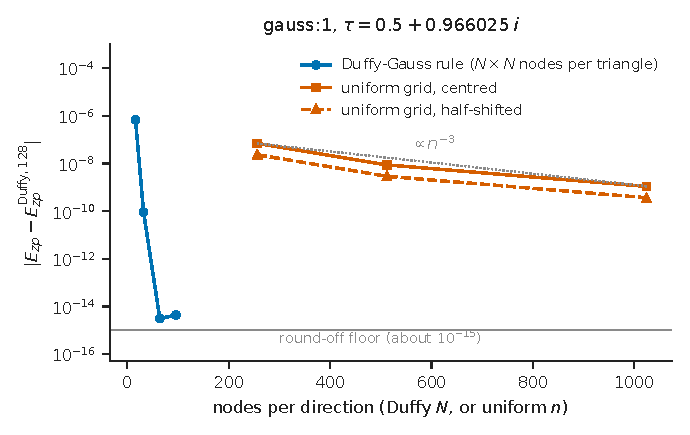
\includegraphics[width=0.62\textwidth]{fig/fig_convergence.pdf}
\caption{Error of the zone integral for \texttt{gauss:1} at $\tau=0.5+0.966025\,i$ against the Duffy $N=128$ value: spectral convergence of the new rule against the $n^{-3}$ grid error
(centred and half-shifted grids); $n^{-3}$ line for reference \tier{X}. Generated by \texttt{make\_figures.py} from \texttt{data/poisson\_check.json}.}\label{fig:conv}
\end{figure}

\paragraph{Controls.} \emph{Positive.} (a) Frozen phonon: the second difference of an independent pair-sum energy of a $5\times5$ supercell (values of $V$ only; for the dipolar potential the Ewald supercell energy) equals
$\tfrac12e^{\mathsf T}De$, max relative difference $\ZPFrozenMax$ over \ZPFrozenN{} cases. (b) Riesz statics against Epstein closed forms agree to $\ZPEpsteinMax$ (and $\ZPEpsteinMaxHi$ for $s\ge4$);
dipolar statics against the Ewald sum to $\ZPDipEwaldMax$. (c) $r_c=400\to800$ changes $\Ezp$ by $\le\ZPCutoffMax$; $\Ezp$ at $\tau,\tau+1,-1/\tau$ agrees to $\le\ZPModularMax$. (d) Poisson $D$ against the explicit real-space sum at 200 random
$\mathbf k$ in 12 cases: $\le\ZPPoissonRealMax$ relative; the exact sum rule against the real-space sum $\le\ZPSumRulePRMax$ and against the Duffy $\langle\tr D\rangle$ $\le\ZPSumRuleDuffyMax$.
(e) An independent numpy implementation of the real-space method (explicit sum, no folding, centred and shifted grids) gives $\ZPIndepGaussTri$ at $\rho$ for \texttt{gauss:1}, against $\ZPEzpTri$.
(f) The static minimiser over the 567 shapes is the triangular lattice for \ZPStaticTriAll{} potentials, as Montgomery's theorem and its Bernstein-mixture extensions predict; a violation would have signalled a code bug.
(g) Stencil Laplacian of $E_{\mathrm{static}}$ and of $\langle\tr D\rangle$ against the exact lattice sum of $h$ (Step~4): $\le2.5\times10^{-10}$ relative for $a\ge0.5$ (ZP-X-0006).
\emph{Negative.} (h) Planted bug, dropping the $-\xi\xi^{\mathsf T}$ term: the real-space match fails by a relative $\ZPBugDropMin$ to $\ZPBugDropMax$; planted $a\leftrightarrow1/a$ swap: invisible at the self-dual $a=1$ ($\ZPBugSwapOneMax$) but
$\ZPBugSwapOtherMin$ to $\ZPBugSwapOtherMax$ elsewhere. (i) The square lattice is flagged unstable for every potential ($\min\lambda/|\mathbf k|^2=\ZPSqUnstable$ for \texttt{gauss:1}). (j) \texttt{gauss:2}, which survives G1, has no stable lower lattice at the \texttt{gauss:1}
competitor shapes ($\Delta\Ezp=\ZPGaussTwoCtl$ at $0.5+0.966\,i$; $0.295+0.9555\,i$ and $0.3+0.9539\,i$ \ZPGaussTwoUnstableA). (k) \emph{Non-completely-monotone potentials.} For attractive Gaussian wells at the square-lattice shell distances
(\texttt{wells:1.0;1.414;0.12;0.5}) the square lattice is a stable static minimiser lower than the triangular one by $\ZPWellsStatic$, and a stable rhombic lattice has $\Ezp$ lower by $\ZPWellsZp$; a second member has the triangular static minimum but a stable lattice $\ZPWellsTwoZp$ lower in $\Ezp$
(Table~\ref{tab:neg}); \texttt{morse:3;1.0} also has a stable competitor ($0.5+0.966\,i$) with lower $\Ezp$ than the triangular lattice, although its static minimiser is triangular. These are \emph{detection-power} controls: they show that the search can find a stable lattice with lower $\Ezp$ when one exists. They are not false-positive controls; that role is played by the survivors (\texttt{gauss:2}, \texttt{gauss:4}, \texttt{gauss:0.25}, \texttt{riesz:6}, for which no stable lower lattice was found, \texttt{gauss:2} in particular at the competitor shapes of \texttt{gauss:1}) and by the frozen-phonon checks of (a).

\begin{table}[t]\centering\footnotesize
\caption{Non-completely-monotone controls (G1, $n=96$, 567 shapes). ``stable'' counts dynamically stable shapes; $\Delta\Ezp$ is the lowest stable competitor against the triangular lattice \tier{X, ZP-X-0009}.}\label{tab:neg}
\begin{tabular}{lcccl}\toprule
potential & tri.\ stable & stable shapes & min $\Delta E_{\mathrm{static}}$ & min $\Delta\Ezp$ (stable)\\\midrule
\tabinput{gen/table_neg.tex}\bottomrule\end{tabular}
\end{table}

\subsection{Result 1: the counterexample}
\begin{table}[t]\centering\footnotesize
\caption{\texttt{gauss:1}, $V=e^{-\pi r^2}$ \tier{X, ZP-X-0001, ZP-X-0004}. $\Ezp$ from the Duffy rule ($N=128$, error about $\ZPQuadErr$); $\min\lambda/|\mathbf k|^2$ over the zone ($|\mathbf k|\ge3\times10^{-3}$);
exact long-wave eigenvalue of the elastic tensor. $\dagger$: marginally stable; not the headline.}\label{tab:head}
\begin{tabular}{lrrrr}\toprule
lattice $\tau$ & $\Ezp$ & $\Delta\Ezp$ & $\min\lambda/|\mathbf k|^2$ & long-wave\\\midrule
\tabinput{gen/table_head.tex}\bottomrule\end{tabular}
\end{table}
For \texttt{gauss:1} the rhombic lattice $\tau=0.5+0.966025\,i$ has $\Delta\Ezp=\ZPdEHead$, i.e.\ $\Ezp=\ZPEzpHead$ against $\ZPEzpTri$ (Table~\ref{tab:head}). It is stable with a clear margin ($\ZPRatioHead$ on the zone,
$\ZPLWHeadExact$ at long wavelength, against $\ZPRatioTri$ and $\ZPLWTriExact$ for the triangular lattice). The G1 grid code at $n=768$ gives $\ZPRustHead$ and $\ZPRustTri$ (differences from the spectral values $\ZPRustDiffHead$, $\ZPRustDiffTri$); the margin is $\ZPMarginRatio$
times the $n=96$ grid error at the triangular point ($\ZPKgridErrOne$). At paper stage the compiled binary reproduced $\ZPRerunEzpHead$ and $\ZPRerunEzpTri$ ($\Delta\Ezp=\ZPRerundE$).
Across all \ZPMapNShapes{} shapes sampled for this potential at $n=96$ (Figure~\ref{fig:map}), \ZPMapNStable{} are dynamically stable; all \ZPMapNLower{} of the \ZPMapNComp{} stable non-triangular shapes have $\Ezp$ below the triangular value
(weakest margin $\ZPMapMaxdE$), so around $\rho$ the triangular lattice is a local \emph{maximum} within the stable region.

\begin{figure}[t]\centering
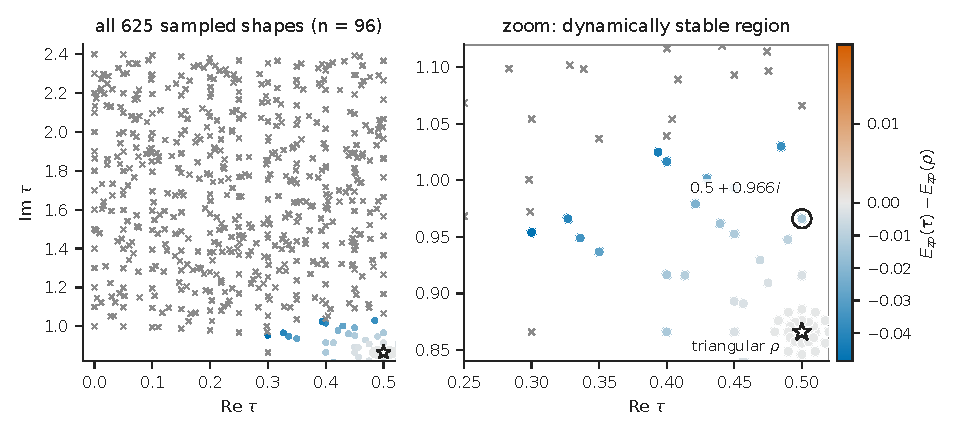
\includegraphics[width=\textwidth]{fig/fig_map.pdf}
\caption{$\Ezp(\tau)-\Ezp(\rho)$ for \texttt{gauss:1} at $n=96$ \tier{X}. Left: all sampled shapes (grey crosses are dynamically unstable). Right: zoom on the dynamically stable region; the star is $\rho$ and the ring is the headline
$0.5+0.966\,i$. Blue is lower than triangular, orange higher (none). Generated by \texttt{make\_figures.py} from the G1 scan files in \texttt{data/}.}\label{fig:map}
\end{figure}

\paragraph{Correction to a G1 figure.} G1 reported its largest margin at $\tau=0.295+0.9555\,i$ ($\Delta\Ezp=\ZPdEMarg$). That value of $\Ezp$ is confirmed (Duffy, $n=768$ and Richardson agree to about $10^{-10}$), but the lattice is
stable only marginally: its exact long-wave eigenvalue is $\ZPMargLW$, $\ZPMargFrac\,\%$ of the triangular value, and the Duffy rule converges slowly there (change $\ZPMargConv$ from $N=96$ to $128$). It is \emph{not} the headline.

\subsection{Result 2: which potentials}
\begin{table}[t]\centering\footnotesize
\caption{Verdicts for the \ZPNTested{} completely monotone potentials \tier{X, ZP-X-0003}. ``Robust min'' is the lowest $\Delta\Ezp$ at $n=384$ among competitors stable on $n=96,192,384$ (candidate points and the dense-scan minima); LW is the exact
long-wave eigenvalue of that competitor as a percentage of the triangular value (-- if not computed); the fifth column is $\Delta\Ezp$ at $0.5+0.966025\,i$ ($n=384$, rc 400). $^\dagger$: for \texttt{gauss:1} the lowest robust competitor is the marginally stable
point $0.295+0.9555\,i$ (long-wave margin 0.06\,\%), which the text demotes (Result~1); the refutation of \texttt{gauss:1} uses $0.5+0.966025\,i$ (fifth column; Tables~\ref{tab:head}, \ref{tab:elastic}). Last column: range over 12 directions at $r=0.01$ of $c=[\Ezp(\tau)-\Ezp(\rho)]y_\rho^2/|\tau-\rho|^2$
(extrapolated in $n$), and the resulting nature of the triangular point.}\label{tab:pot}
\begin{tabular}{lrrrrll}\toprule
potential & robust min $\Delta\Ezp$ & at $\tau$ & LW\,\% & at $0.5{+}0.966i$ & verdict & $c$ at $\rho$\\\midrule
\tabinput{gen/table_potentials.tex}\bottomrule\end{tabular}
\end{table}
QU-1 is refuted for \ZPNRefuted{} of \ZPNTested{} (\ZPListRefuted) by a stable lattice with lower $\Ezp$; it is not refuted for \ZPListSurvive{} on the 567-point scan and the dense paths, where the triangular lattice is a strict local minimum of $\Ezp$
(an evidence statement from a sample and two one-dimensional paths, not an exhaustive search). Of the eight refutations, \ZPNTwoComp{} also have a stable competitor below the triangular lattice at $0.5+0.966\,i$; the exception is \ZPNoTwoComp, whose refutation rests on one competitor ($0.3+0.954\,i$) with a small
long-wave margin (0.08\,\% of the triangular value, Table~\ref{tab:pot}) and whose triangular point is a local minimum of $\Ezp$ ($c>0$); it is the weakest of the eight. The competitors at $x=0.3$ for the dipolar, Riesz and Yukawa
potentials have long-wave margins of 0.1\,\% to 1.5\,\% of the triangular value (Table~\ref{tab:elastic}); their finite-$\mathbf k$ stability rests on the G1 grids ($n$ up to 384), since the Poisson method is Gaussian-only. The refutation of ``every completely monotone $g$'' needs one potential, and
\texttt{gauss:1} is verified by independent methods. Stable lattices form a small neighbourhood of $\rho$ (within about $\ZPMaxStableDist$ in $\tau$ at $n=96$).
Several lowest $n=96$ competitors (\texttt{gauss:0.5} at $0.3+0.954\,i$, \texttt{yukawa:1} at $0.295+0.9555\,i$, \texttt{riesz:3} at $0.5+1.036\,i$) turned unstable on finer grids and were dropped; the first two are long-wave unstable ($\ZPDroppedGaussHalf$, $\ZPDroppedYuk$), consistent with dropping them.

\begin{table}[t]\centering\footnotesize
\caption{Exact long-wave limit $\min_t\lambda_{\min}C(t)$ (no $\mathbf k$-grid; $r_c=200$ and $400$ agree to $\le\ZPElasticRcDiff$) for one competitor sufficient for each refutation, the triangular lattice and the square lattice \tier{X, ZP-X-0003}.
The competitor is the robust minimum of Table~\ref{tab:pot} for every potential except \texttt{gauss:1}, where that minimum is the demoted marginal point $0.295+0.9555\,i$ and the table uses $0.5+0.966\,i$ instead.}\label{tab:elastic}
\begin{tabular}{lcrrr}\toprule
potential & competitor $\tau$ & competitor & triangular & square\\\midrule
\tabinput{gen/table_elastic.tex}\bottomrule\end{tabular}
\end{table}

\subsection{Result 3: curvature at the triangular point, and the Gaussian family}
For $V=e^{-\pi ar^2}$ the curvature $c(a)=\tfrac14\Delta\Ezp(\rho)$ (Step~6) is numerically negative, that is, the triangular lattice is a strict local \emph{maximum} of $\Ezp$, on $a\in(\ZPRootOne,\ZPRootTwo)$ within the range $0.15\le a\le4$. The sign changes were located by a scan of 23 values of $a$ ($0.1$ to $8$) and bisected
(roots robust to the quadrature node count and the stencil step); the scan does not exclude further sign changes between its points, and at the roots themselves $c=0$ and the second-order test is inconclusive. It contains the refuted \texttt{gauss:0.5} ($c=\ZPcHalf$) and \texttt{gauss:1} ($c=\ZPcOne$); the survivors lie outside ($\ZPcQuarter$, $\ZPcTwo$, $\ZPcFour$ at $a=\tfrac14,2,4$). The real-space Rust code at $n=768$
confirms both sign changes independently: $\Ezp(\rho\pm0.02)-\Ezp(\rho)=\ZPBrOne$ at $a=0.35$, $\ZPBrTwo$ at $0.40$, $\ZPBrThree$ at $1.50$ and $\ZPBrFour$ at $1.65$. At $\rho$, for the four Gaussians with $a\ge0.5$ of the mechanism study ($a=0.5,1,2,4$), $\partial_{xx}\Ezp=\partial_{yy}\Ezp$ to $\ZPIsoRelMax$ relative, $|\partial_{xy}\Ezp|\le\ZPIsoXYMax$ and $|\nabla\Ezp|\le\ZPIsoGradMax$, as Step~6 predicts.
At $a=0.25$, near the soft-shear region, the relative difference is $\ZPIsoRelQuarter$ and $|\nabla\Ezp|\approx\ZPIsoGradQuarter$ (the finite-difference stencil is less accurate there).
Table~\ref{tab:curv} also lists $\Delta\langle\tr D\rangle(\rho)$ from the exact lattice sum of Step~4; its sign changes at $a=\ZPRootLapm$, consistent with Luo--Wei ($a\le1$) and with the assertion, quoted by Luo and Wei from B\'etermin~\cite{betermin}, that the hexagonal optimality of $S(\alpha;\cdot)$ cannot hold for all $\alpha>0$
(here it fails locally for $\alpha<0.914$). \textbf{The sum rule alone does not fix the sign of $c$}: they differ on about $(0.12,0.38)$ and $(1.09,1.58)$ (Figure~\ref{fig:curv}).
\begin{figure}[t]\centering
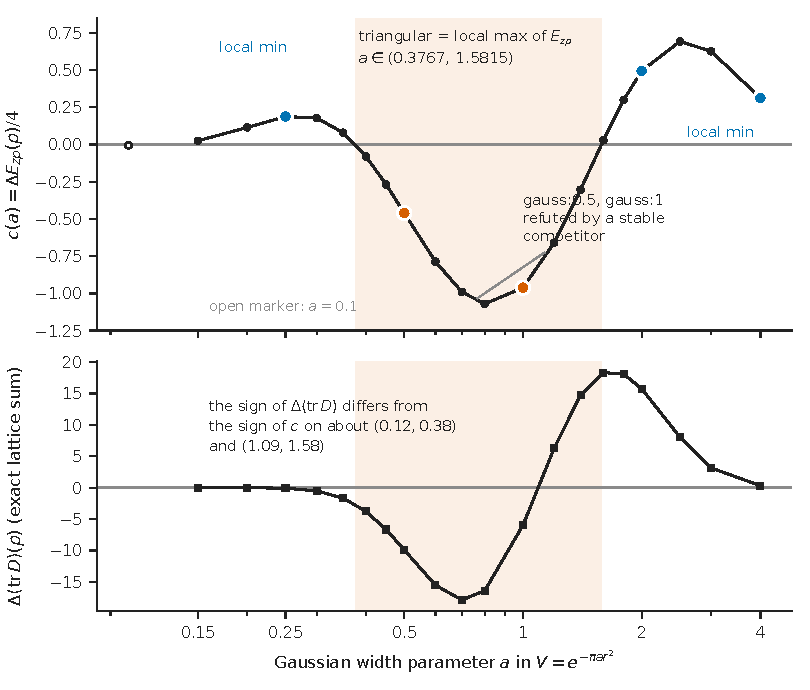
\includegraphics[width=0.78\textwidth]{fig/fig_curvature.pdf}
\caption{Top: $c(a)=\Delta\Ezp(\rho)/4$ for $V=e^{-\pi ar^2}$ \tier{X}; shaded: $c<0$, the triangular lattice is a local maximum of $\Ezp$. Filled markers are the five Gaussians of the G1 scan (orange: refuted). Bottom: $\Delta\langle\tr D\rangle(\rho)$, the exact lattice sum of Step~4 \tier{X, with Tier~A formula}.
Generated by \texttt{make\_figures.py} from \texttt{data/mechanism.json}.}\label{fig:curv}
\end{figure}
\begin{table}[t]\centering\footnotesize
\caption{$c(a)$, the curvature of $\langle\tr D\rangle$ from the exact lattice sum, and the smallest $\lambda/|\mathbf k|^2$ of the triangular lattice, for $V=e^{-\pi ar^2}$ \tier{X, ZP-X-0005}. $^\dagger$ the triangular lattice is
marginal (shear eigenvalue $\le1.5\times10^{-9}$ for $a\le0.123$, $3.3\times10^{-12}$ at $0.1$; harmonic picture doubtful; $c$ changes sign again near $a\approx\ZPRootA$, uncertain by about $10^{-3}$ since the quadrature rules shift $c$ by $10^{-5}$ there).
$^\ddagger$ precision-flagged: the Poisson form loses relative accuracy when $\Ezp$ is tiny; at $a=8$ the triangular lattice failed the stability test.}\label{tab:curv}
\begin{tabular}{lrrr|lrrr}\toprule
$a$ & $c$ & $\Delta\langle\tr D\rangle$ & $\min\lambda/k^2$ & $a$ & $c$ & $\Delta\langle\tr D\rangle$ & $\min\lambda/k^2$\\\midrule
\tabinput{gen/table_curv.tex}\bottomrule\end{tabular}
\end{table}

\subsection{Result 4: where the energy is lost}
Finite-difference decomposition (Step~8) at $a=1$ gives $\Delta\Ezp(\rho)=\ZPLapOne=\mathrm{Lin}\,(\ZPLinOne)+\mathrm{Conc}\,(\ZPConcOne)$, with $\ZPShellFracOne\,\%$ from the outer (zone-boundary) shell of the Duffy map; $\mathrm{Lin}+\mathrm{Conc}$ matches the stencil Laplacian to $\ZPDecompResid$.
At $a=0.25$ and $2$ a large positive $\mathrm{Lin}$ beats $\mathrm{Conc}$ (Table~\ref{tab:decomp}). For the headline competitor the loss is a \emph{softening of the lower branch near the zone boundary}
($\ZPSplitLowerZB$ of $\ZPSplitLower$; long-wave shell $\ZPSplitLowerLW$), partly offset by the upper branch ($\ZPSplitUpper$) (Figure~\ref{fig:split}). The mean-square frequency falls by $|\ZPSplitDtrD|$, which moves the Einstein bound by only $\ZPSplitEinstein$
($\ZPSplitEinsteinPct\,\%$ of the gain); the other $\ZPSplitJensenPct\,\%$ ($\ZPSplitJensen$) is the Jensen gap, a wider spread of the spectrum. The negative control \texttt{gauss:2} at the same shape has $\langle\tr D\rangle$ rising by $\ZPSplitTwoDtrD$, the upper branch gaining $\ZPSplitTwoUpper$, and a net $\ZPSplitTwoTotal$.
These are Tier~X numbers with a Tier~C reading (zone-boundary softening of the shear branch; ZP-X-0007, ZP-C-0009): the mechanism was not tested separately.
\begin{figure}[t]\centering
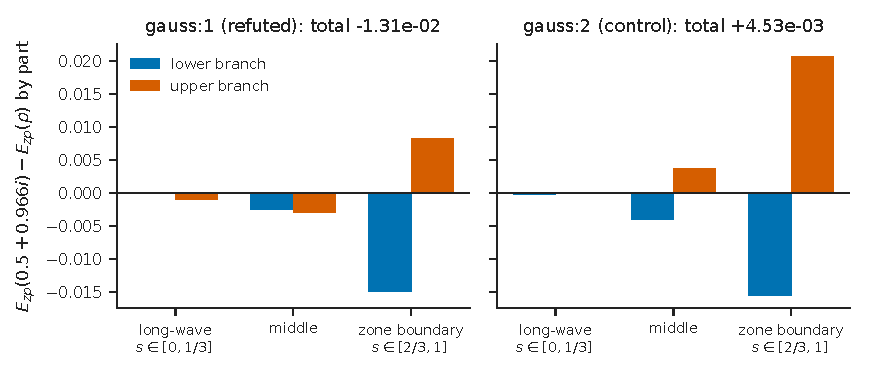
\includegraphics[width=0.85\textwidth]{fig/fig_split.pdf}
\caption{$\Ezp(0.5+0.966\,i)-\Ezp(\rho)$ split by branch and by zone shell (Duffy radial thirds) \tier{X}; left the refuted \texttt{gauss:1}, right the control \texttt{gauss:2}. Generated by \texttt{make\_figures.py} from \texttt{data/mechanism.json}.}\label{fig:split}
\end{figure}
\begin{table}[t]\centering\footnotesize
\caption{Decomposition of $\Delta\Ezp(\rho)$ into linear response and concavity (diagonal and branch-mixing parts), and the curvature of the Einstein bound \tier{X, ZP-X-0007}.}\label{tab:decomp}
\begin{tabular}{rrrrrrr}\toprule
$a$ & $\Delta\Ezp$ & Lin & Conc & Conc (diag) & Conc (cross) & $\Delta E_{\mathrm{Einstein}}$\\\midrule
\tabinput{gen/table_decomp.tex}\bottomrule\end{tabular}
\end{table}

\subsection{Result 5: the full functional \texorpdfstring{$E_{\mathrm{static}}+\Lambda\Ezp$}{E\_static + Lambda E\_zp}}
With $V\to\epsilon V$, $E_{\mathrm{static}}$ scales as $\epsilon$ and $\Ezp$ as $\sqrt\epsilon$, so the physical family is $E_{\mathrm{static}}+\Lambda\Ezp$ with $\Lambda\propto\epsilon^{-1/2}$ (ZP-X-0010). Over the stable sample the triangular lattice stops being the minimiser at some
$\Lambda\in[\ZPLambdaFirstMin,\ZPLambdaFirstMax]$ for every refuted potential (for \texttt{riesz:4} only at $\Lambda=10$), and remains the minimiser for the survivors at all five $\Lambda\in\{0.1,0.3,1,3,10\}$. The harmonic approximation fails for large $\Lambda$ (strong quantum motion, melting), so this
is a statement about the functional only. Moreover the competitors are \emph{not stress-free}: the triangular lattice has the lower static energy, so each competitor is held in shape by a constraint; a statement about $E_{\mathrm{total}}$ at its own equilibrium shape is a different statement and is untested.

\subsection{The rusty-SUNDIALS improvement}
The lane added \texttt{phonon.rs} (the lattice-phonon module: real-space $D(\mathbf k)$, folded-grid $\Ezp$, stability, Epstein/Ewald statics; 12 unit tests according to the lane, incl.\ a regression of the headline and a negative control) and, in this stage's commit \texttt{\ZPRustySpectralShort}, \texttt{phonon\_spectral.rs}
(280 lines): Gauss--Legendre nodes, \texttt{GaussPoisson} (reciprocal-space Gaussian dynamical matrix with the exact sum rule), \texttt{ezp\_gauss\_duffy} (the spectral zone rule) and \texttt{curvature\_at\_rho\_gauss}; plus the \texttt{lattice\_phonon} subcommands
\texttt{duffy} and \texttt{curv}. The spectral rule replaces an $n^{-3}$ grid error (about $10^{-6}$ at $n=96$) by about $\ZPQuadErr$ at $N=128$ (Figure~\ref{fig:conv}), which makes the sign of $c(a)$ resolvable to its roots and
turned a numerical refutation into one whose margin is about $10^{12}$ times the quadrature error (the remaining uncertainty is modelling: the harmonic approximation). Five new unit tests cover Gauss--Legendre exactness, Poisson against real-space $D$ at three shapes to $10^{-12}$, Duffy against Richardson grids, a regression of the
headline with the square lattice as negative control, and the sign of $c$ at $a=0.25,1,2$. At paper stage (same pipeline, \texttt{data/rerun\_*}): \texttt{cargo test -p qf-yukawa-crystal}: \ZPCargoPassed{} passed, \ZPCargoFailed{} failed, \ZPCargoIgnored{} ignored;
\texttt{cargo clippy --workspace --features experimental -- -D warnings}: no warnings or errors; \texttt{cargo fmt --check}: clean; \texttt{lattice\_phonon curv 1 48 0.002} gives $c=\ZPRerunC$. After the audit (hardening point N7) commit \texttt{\ZPRustyHardenShort} added \texttt{ezp\_gauss\_duffy\_stable} and \texttt{DuffyResult::is\_stable}, so that the clipped $\Ezp$ of an unstable shape (which the unchecked rule returns, favouring the unstable lattice) cannot be used by accident,
and doc comments saying so; no existing function changed behaviour, one test was added (stable shape returns the same energy, the square lattice returns \texttt{None}); \texttt{cargo test -p qf-yukawa-crystal}: \ZPReviseCargoPassed{} passed, \ZPReviseCargoFailed{} failed, \ZPReviseCargoIgnored{} ignored; fmt and clippy clean (\texttt{data/revise\_cargo\_*.txt}). The reported numbers were all produced before this commit. No LeanFlow change was made in this lane.

%=====================================================================
\section{A restricted conjecture, QU-1$'$}\label{sec:qu1p}
\textbf{QU-1$'$ \tier{X-supported conjecture, not proved}.} For $g_a(t)=e^{-\pi at}$ with $0.15\le a\le4$, the triangular lattice is a strict local minimiser of $\Ezp$ among unit-covolume planar Bravais lattices if $a<\ZPRootOne$ or $a>\ZPRootTwo$, and a strict local maximiser (so not a minimiser) for $\ZPRootOne<a<\ZPRootTwo$; the numerical $c$ of Table~\ref{tab:curv} is negative there.
The endpoints $a_1=\ZPRootOne$ and $a_2=\ZPRootTwo$ are bisected numerical roots of $c$; at $c=0$ the second-order test is inconclusive, so nothing is stated at the endpoints, and the roots carry the uncertainty of a floating-point scan.
It is suggested by Table~\ref{tab:curv} and supported by the $n=768$ cross-check; nothing proves it. Caveats kept outside the statement: at $a=0.15$ the triangular lattice is barely stable ($\min\lambda/|\mathbf k|^2=\ZPSmallaAFifteenRatio$); below $a\approx\ZPRootA$ the sign of $c$
changes again at a marginal lattice; $a=6,8$ are precision-flagged. The global version (triangular is the $\Ezp$ minimiser among dynamically stable lattices for $a>\ZPRootTwo$) is supported only by the G1 sample at $a=2,4$ and is open. A proof would need rigorous bounds on the $\mathrm{Lin}$ and $\mathrm{Conc}$ integrals,
for instance by interval arithmetic over the Duffy rule; $\Delta\Ezp(\rho)$ has no theta-function closed form because $\Ezp$ is not a pair sum. This was not attempted.

%=====================================================================
\section{Claim ledger}\label{sec:ledger}
\texttt{ledger/build\_ledger.py} files \ZPLedgerN{} claims: \ZPLedgerA{} at Tier~A, \ZPLedgerL{} at L, \ZPLedgerC{} at C and \ZPLedgerX{} at X. Each has a content-addressed evidence blob in \texttt{ledger/evidence/}: verbatim axiom lines and source hashes (A), the quotation with the Elenchus citation-gate result (L),
the argument text (C), and result files with \texttt{claim\_licence: false} (X). The tier discipline of \texttt{tools/ledger.py} (a claim may not sit above anything it depends on) forces everything resting on a floating-point result to X:
the sum-rule consequences that combine Luo--Wei with a Poisson identity are filed at C, not L; the mechanism reading, the roots $a_1,a_2$ and QU-1$'$ are filed at X, not C. The gate
(\texttt{tools/ledger.py ledger.json -{}-evidence-dir evidence}, verbatim output in \texttt{ledger/gate\_output.txt}) exits with code~\ZPGateExit. It reports \textbf{\ZPGateBlock{} blocking findings} and \textbf{\ZPGateFlag{} flags}
(\ZPGateFlagKinds, one per Tier~A row: no person has certified that the Lean statements mean what their glosses say). The flags remain open. The Elenchus citation gate (\texttt{tools/citation\_check.py}) \emph{accepted} \ZPCitationAccepted{} of \ZPCitationN{} quotations (tier ceiling~L);
the quotations were copied programmatically from \texttt{pdftotext} output of the arXiv PDFs, so the gate tests fidelity to the fetched text, while ``statement match'' is the agent's own judgement. Montgomery's theorem is cited through Deng--Luo~\cite{dengluo}; the original paper was not opened.

%=====================================================================
\section{Limitations}\label{sec:lim}
\begin{itemize}\itemsep=1pt
\item \textbf{Everything about $\Ezp$ is Tier~X or~C.} The refutation is floating-point: robust (four implementations, stable on grids to $n=384$ and by the exact long-wave limit, frozen-phonon agreement $\ZPFrozenMax$), but not a Lean statement and not an interval-arithmetic enclosure. A certified enclosure of $\Ezp$ at the two shapes would upgrade it and is the natural next step; it was not done.
\item \textbf{Harmonic, Bravais, two-dimensional only.} Nothing is said about non-Bravais structures (the harder QU-2), anharmonic corrections, quantum melting or the true quantum ground state; these matter most where the shear eigenvalue is tiny (small $a$, marginal points).
\item \textbf{Competitors are not stress-free.} See Result~5. QU-1 as stated compares a functional over imposed shapes and is refuted regardless; $E_{\mathrm{total}}$ at equilibrium shape is untested.
\item \textbf{Sample, not exhaustive search.} The survivors rest on 567 shapes plus two dense paths; the refutations rest on competitors sampled near $\rho$. We do not claim any listed point is the global minimiser of $\Ezp$.
\item \textbf{Stability margins.} $n=96$ stability is optimistic near the edge. The $x=0.3$ competitors have small long-wave margins; \texttt{riesz:4} rests on a single such point. Finite-$\mathbf k$ stability of the non-Gaussian competitors rests on G1's grids.
\item \textbf{Excluded potentials.} Coulomb and Keldysh (neutralising background, plasmon $k\to0$) are not covered. The harmonic zero-point energy of unit-amplitude potentials with $\hbar=m=1$ only rescales; the sign of $\Delta\Ezp$ does not depend on units.
\item \textbf{Post-hoc analysis.} The curvature scan, the mechanism and QU-1$'$ were run after G1 refuted the conjecture and were not preregistered. The mechanism (zone-boundary softening) is interpretation.
\item \textbf{Novelty.} One alphaXiv search found no paper on lattice-shape optimality of the harmonic zero-point energy: this is absence by one search, not a claim of novelty.
\item \textbf{Verification status.} No human audit of this preprint, of the Lean module, or of the Rust code. One separate AI audit exists, with the scope of Section~\ref{sec:audit}: several results (the dipolar, Riesz and Yukawa refutations, the long-wave elastic tensor, the Lin/Conc split, Result~5, $c(a)$ beyond its sign at $a=1,2$, and the 691 lines of \texttt{phonon.rs}) were checked only through the producer's data and tests. The paper-stage reruns are by the same pipeline. The seed detector could not run. Nothing here rests on openai/math (AI-generated, not peer reviewed), except that its toolchain compiles the Lean file.
\item \textbf{Literature.} Montgomery's 1988 paper and B\'etermin's 2016 paper were not opened; both are cited second-hand through arXiv texts of Luo--Wei and Deng--Luo. The Luo--Wei journal version (J.\ Math.\ Phys.\ 65 (2024) 071901, as listed in Deng--Luo, ref.~[27]) was not opened; we cite the arXiv text.
\end{itemize}

%=====================================================================
\section{Separate AI audit: scope and result}\label{sec:audit}
After the paper stage, a separate AI agent (Claude; it wrote none of the paper, the Lean module, the Rust code or the analysis) audited the preprint; the report is \texttt{AUDIT.md}, its verdict is ``accept with corrections'' with no blocking finding, and
the corrections were applied (\texttt{REVISION.md}). It is a producer~$\neq$~verifier check at the agent level only; \textbf{no human audit exists}, and the eight open Tier~A ledger flags stay open because an AI adequacy review is not a person's certification.
\emph{Recomputed with the auditor's own code:} the Lean module (recompiled with the pinned stack, 19 printed declarations plus the helper \lean{rho\_ne\_zero} within the allowlist; the auditor's own planted \lean{sorry} and planted axiom were caught by \lean{\#print axioms}; the stated derivatives are Mathlib's \lean{deriv}; the hypothesis of the inversion lemma is satisfiable);
$\Ezp$ of \texttt{gauss:1} at $\rho$ and at $0.5+0.966025\,i$ by an independent real-space code sharing no code with the producer (agreement to about $10^{-12}$, invariance under $\tau\mapsto-1/\tau$), stability signs of the triangular, rhombic and square lattices, and the sign and size of $c$ at $a=1,2$;
the \texttt{gauss:0.5} refutation at $(0.5,1.016)$; the map recount of \texttt{gauss:1}; all generated macros and tables by regenerating them from \texttt{data/}; the three citations against the arXiv PDFs (the citation gate accepted all three); the crate tests, \texttt{cargo fmt} and clippy.
\emph{Checked only through the producer's data or tests, not recomputed:} the dipolar, Riesz and Yukawa refutations, the exact long-wave elastic tensor, the Lin/Conc decomposition, Result~5, $c(a)$ beyond its sign at $a=1,2$, and \texttt{phonon.rs}.
The audit's reproduction of the ledger gate gave 0 blocking findings and 8 flags, as in Section~\ref{sec:ledger}.

%=====================================================================
\section{Reproducibility}\label{sec:repro}
AutoevolveAI: branch \texttt{worktree-openai-math-discovery}, HEAD below; the new files (this paper, the Lean module, the G2 result files) were uncommitted when the PDF was built and are committed by the release procedure, not by this revision; the cited hashes of the Lean files below identify their content. Lean sha256 values are in Section~\ref{sec:lean}.
\begin{itemize}\scriptsize\itemsep=0pt\item AutoevolveAI HEAD: \texttt{9d245742c1655852103abb28f585e21af54851e6}\end{itemize}
rusty-SUNDIALS branch \texttt{physics/p2-zero-point-optimality-2026-10-25}, local, not pushed:
\begin{itemize}\scriptsize\itemsep=0pt
\item \texttt{\ZPRustyGate} (lattice-phonon module and falsification gate);
\item \texttt{\ZPRustyEdge} (stability-edge verification, dense scans);
\item \texttt{\ZPRustySpectral} (spectral zone rule, curvature, G2 checks);
\item \texttt{\ZPRustyHarden} (post-audit hardening: \texttt{ezp\_gauss\_duffy\_stable}, no change to any reported number).
\end{itemize}
\begin{lstlisting}[basicstyle=\ttfamily\scriptsize]
taskset -c 4-7 python3 scripts/certified_numerics/lean_pinned.py compile formal_cert/Programmes/ZeroPoint/Basic.lean \
  --olean Programmes.ZeroPoint.Basic --json-out papers/prog_zero_point_optimality/data/rerun_basic.json
taskset -c 4-7 python3 scripts/certified_numerics/lean_pinned.py compile formal_cert/Programmes/ZeroPoint/Controls.lean --json-out .../rerun_controls.json
CARGO_TARGET_DIR=... cargo test --release -j 2 --offline -p qf-yukawa-crystal -- --test-threads=2
CARGO_TARGET_DIR=... cargo clippy -j 2 --offline --workspace --features experimental -- -D warnings
lattice_phonon duffy 1 0.5 0.966025403784 64 ; lattice_phonon curv 1 48 0.002
python -I phonon_poisson_check.py | phonon_elastic_check.py | phonon_mechanism.py | phonon_smalla_check.py | phonon_sumrule_identity.py   # crates/qf-yukawa-crystal/scripts
python -I papers/prog_zero_point_optimality/human_check.py ; make_figures.py ; ledger/build_ledger.py ; ledger/run_gate.py ; gen_inputs.py ; pdflatex main.tex (twice)
\end{lstlisting}
All numbers in this paper are generated into \texttt{gen\_numbers.tex} and \texttt{gen/} from the files in \texttt{data/}, which are copies of the lane's results in \texttt{results/programmes/2026-10-25/P2/} (\texttt{GATE.md}, \texttt{PROOF.md}).

\begin{thebibliography}{99}\small
\bibitem{mont} H.~L. Montgomery, \emph{Minimal theta functions}, Glasgow Math.\ J.\ 30 (1988) 75--85. Cited second-hand through~\cite{dengluo}, p.~3, Theorem~A; the original was not opened.
\bibitem{dengluo} K.~Deng, S.~Luo, \emph{Minimizing lattice energy and hexagonal crystallization}, arXiv:2411.17199v1 (2024). Accessed 2026-10-25; Theorem~A quoted and gate-checked.
\bibitem{luowei} S.~Luo, J.~Wei, \emph{On lattice hexagonal crystallization for non-monotone potentials}, arXiv:2302.05042v1 (2023); journal version J.\ Math.\ Phys.\ 65 (2024) 071901 (listed as ref.~[27] of~\cite{dengluo}; not opened). Accessed 2026-10-25; Corollary~1.1 (p.~3) and Lemma~3.5 (p.~12) quoted and gate-checked. SHA-256 of the fetched texts: \texttt{ledger/sources/MANIFEST.md}.
\bibitem{betermin} L.~B\'etermin, \emph{Two-dimensional theta functions and crystallization among Bravais lattices}, SIAM J.\ Math.\ Anal.\ 48(5) (2016) 3236--269 (pages exactly as printed in~\cite{luowei}, ref.~[7]); cited only as described by Luo--Wei (their pp.~2--3, where Subsection~4.3 of B\'etermin, p.~3249, is referred to); not opened.
\bibitem{ar} X.~Callens, five autoresearch preprints on triangular-lattice corollaries and consistency studies: doi:10.5281/zenodo.23646103 (dipolar excitons), 23646105 (Yukawa), 23646107 (Rytova--Keldysh),
23646111 ($\sigma=3$ dyadic shell model), 23646117 (Bogoliubov structure factor) (2026).
\bibitem{txt} X.~Callens, \emph{The Triangular Lattice and Universal Optimality} (textbook), doi:10.5281/zenodo.23295142 (2026).
\end{thebibliography}
\noindent This preprint applies the approach of~\cite{ar,txt} (kernel-checked consequences, Elenchus tiers, rusty-SUNDIALS consistency studies) to the zero-point functional and reports a negative result.
\end{document}
